%% 
%% Copyright 2019-2021 Elsevier Ltd
%% 
%% This file is part of the 'CAS Bundle'.
%% --------------------------------------
%% 
%% It may be distributed under the conditions of the LaTeX Project Public
%% License, either version 1.2 of this license or (at your option) any
%% later version.  The latest version of this license is in
%%    http://www.latex-project.org/lppl.txt
%% and version 1.2 or later is part of all distributions of LaTeX
%% version 1999/12/01 or later.
%% 
%% The list of all files belonging to the 'CAS Bundle' is
%% given in the file `manifest.txt'.
%% 
%% Template article for cas-sc documentclass for 
%% single column output.

\documentclass[a4paper,fleqn]{cas-sc}

% If the frontmatter runs over more than one page
% use the longmktitle option.

%\documentclass[a4paper,fleqn,longmktitle]{cas-sc}

\usepackage[numbers]{natbib}
%\usepackage[authoryear]{natbib}
%\usepackage[authoryear,longnamesfirst]{natbib}
\usepackage{graphicx}
\usepackage{multirow}
\usepackage[normalem]{ulem}
\useunder{\uline}{\ul}{}
\usepackage{lscape}
\usepackage{longtable}
\usepackage{booktabs,tabularx}
\usepackage{float}

%%%Author macros
\def\tsc#1{\csdef{#1}{\textsc{\lowercase{#1}}\xspace}}
\tsc{WGM}
\tsc{QE}
%%%

% Uncomment and use as if needed
%\newtheorem{theorem}{Theorem}
%\newtheorem{lemma}[theorem]{Lemma}
%\newdefinition{rmk}{Remark}
%\newproof{pf}{Proof}
%\newproof{pot}{Proof of Theorem \ref{thm}}

\begin{document}
\let\WriteBookmarks\relax
\def\floatpagepagefraction{1}
\def\textpagefraction{.001}

% Short title
\shorttitle{Classification of Culinary Vegetable Images Using Deep Learning Models}    

% Short author
\shortauthors{C. Kumar}  

% Main title of the paper
\title [mode = title]{Classification of Culinary Vegetable Images Using Deep Learning Models}  


\begin{comment}
% Title footnote mark
% eg: \tnotemark[1]
\tnotemark[<tnote number>] 

% Title footnote 1.
% eg: \tnotetext[1]{Title footnote text}
\tnotetext[<tnote number>]{<tnote text>} 

% First author
%
% Options: Use if required
% eg: \author[1,3]{Author Name}[type=editor,
%       style=chinese,
%       auid=000,
%       bioid=1,
%       prefix=Sir,
%       orcid=0000-0000-0000-0000,
%       facebook=<facebook id>,
%       twitter=<twitter id>,
%       linkedin=<linkedin id>,
%       gplus=<gplus id>]

\author[<aff no>]{Chandan Kumar}[<options>]

% Corresponding author indication
\cormark[<corr mark no>]

% Footnote of the first author
\fnmark[<footnote mark no>]

% Email id of the first author
\ead{chandanksindhiya@gmail.com}

% URL of the first author
\ead[url]{<URL>}

% Credit authorship
% eg: \credit{Conceptualization of this study, Methodology, Software}
\credit{<Credit authorship details>}

% Address/affiliation
\affiliation[<aff no>]{organization={Mahatma gandhi central university Bihar},
            addressline={Motihari}, 
            city={Motihari},
%          citysep={}, % Uncomment if no comma needed between city and postcode
            postcode={845401}, 
            state={Bihar},
            country={India}}

\author[<aff no>]{<Chandan Kumar>}[<options>]

% Footnote of the second author
\fnmark[2]

% Email id of the second author
\ead{}

% URL of the second author
\ead[url]{}

% Credit authorship
\credit{}

% Address/affiliation
\affiliation[<aff no>]{organization={Mahatma gandhi central university Bihar},
            addressline={Motihari}, 
            city={Motihari},
%          citysep={}, % Uncomment if no comma needed between city and postcode
            postcode={845401}, 
            state={Bihar},
            country={India}}

% Corresponding author text
\cortext[1]{Chandan Kumar}

% Footnote text
\fntext[1]{}

% For a title note without a number/mark
%\nonumnote{}


\end{comment}



% Here goes the abstract
\begin{abstract}
Due to their abundance in calcium, vitamins, and minerals, vegetables are known to have a wide range of health benefits for the human body, and several studies on their nutritional worth have been carried out. One must be able to precisely recognise and classify each vegetable in order to completely understand its subtleties, which is a challenging process. The use of deep learning techniques and several complex models has greatly improved this activity. Well-known deep learning models including Resnet, Vgg, Alexnet, Squeezenet, Shufflenet, Googlenet, Densenet, and Resnet50 are used in this discipline. In order to automate vegetable identification, these models are made to separate and group a variety of vegetable characteristics and properties.The effectiveness of these deep learning models is ultimately determined by their precision after training. The more accurately the model can categorise and detect vegetables, the more accurate it will be. One model, the Resnet50, has emerged as a standout performer after extensive analysis and testing. It has proven to have a record of 0.999333\% accuracy that is unequalled. Due to its remarkable accuracy, which surpasses that of all other classifiers examined, Resnet50 is the best choice for precisely categorising and recognising vegetables.The abundance of health advantages provided by vegetables, in conclusion, emphasises the significance of precise identification and classification. This approach has undergone a revolution because to deep learning, which uses models like Resnet50 to achieve accuracy rates that are higher than any others. As a result, we are better equipped to recognise and utilise the nutritive potential of vegetables for human welfare.

\end{abstract}


\begin{keywords}
 \sep Classification \sep performance \sep Culinary Vegetable \sep Image Preprocessing \sep RGB Image \sep Deep Learning
\end{keywords}

\maketitle

% Main text
\section{Introduction}
Agriculture is essential to existence and plays a significant part in daily activities. As a source of energy and a remedy for health issues, vegetables are important to our lives \cite{toor2021nutrients}.  Therefore, it is essential to quickly and precisely identify gourmet veggies. Their primary responsible administrator's potential, which can be either overpowering or non-irresistible, can be used to comprehensively assemble culinary vegetablesTo recognise different veggies, Deep Learning algorithm methods are applied \cite{tripathi2021detection}.Deep Learning \cite{kaur2022optimization} uses its scope to perform image recognition. Shape, size, colour, veining, and sap are just a few of the characteristics of vegetables that are examined to determine their classification. Images of numerous culinary vegetables are gathered from various locations and fitted to the machine for the application of deep learning models. he models are put to the test after training, and their performance is assessed.
        
            With the aid of precision, \cite{agarwal2021classification}.The classification of culinary vegetables is being done using supervised models as Resnet, Vgg, Alexnet, Squeezenet, Shufflenet, Googlenet, Densenet, and Resnet50 \cite{rocha2010automatic}.Multiple pixels that are represented across height and breadth make up an image. Pixels can be RGB or Grayscale \cite{padmavathi2016implementation}. Pixel values in grayscale range from 0 to 255, with 0 being black and 255 denoting white. Red, green, and blue hue intensities are represented by the RGB pixel's three integers, which have values between 0 and 255. RGBA is an improved variant of RGB in which the alpha field is contained in A. Once we have an understanding of the image, we may discuss image processing \cite{egmont2002image}. The image is transformed during image processing into a digital format so that specific operations can be carried out \cite{salvi2021impact}. It displays the 2D signal representation when different techniques are used. The features of image processing include retrieval, sharpening, pattern recognition, visualization, and recognition \cite{behura2021cluster}.
           Several steps are involved in image processing. Image is the first stage of image processing, during which the image is preprocessed. Enhancement of images focuses on contrast and brightness. Image restoration eliminates noise and improves appearance. Image compression is used to shrink the size of the image in order to permit data fading \cite{valikhani2021machine}. After has gathered a dataset of 15 categories, with a minimum of 828 photos in each category. The photographs, which were taken in a range of fields, underwent image augmentation using the technology. Each image has a size of 250 by 250. The market, the farm, and Krishi Vigyan Kendra are where the culinary photos are gathered.  The vibrant images were captured with a 16MP phone camera. Classifiers were used after this data were saved as a dataset. The photos are all resized to 224 X 224 before being simultaneously cropped using a batch image cropper. Then, several models are used to achieve the required classification outcomes.
           Given the tremendous health advantages of vegetables, the problem statement in this instance focuses on the urgent need for accurate vegetable identification and classification. Deep learning methods, particularly Resnet50, which achieves the highest levels of accuracy and makes it possible to better use the nutritional potential of vegetables for human well-being, have significantly improved this procedure. To assure originality and prevent plagiarism, this statement was carefully crafted.

           This study seeks to create a dataset of numerous photographs of gourmet vegetables and preprocess the dataset using a variety of methods, including model training and selection. Deep learning methods (such Resnet, Vgg, Alexnet, Squeezenet, Shufflenet, Googlenet, Densenet, and Resnet50) are trained on vast amounts of training labelled data, and the effectiveness of each classifier is then assessed using the DL algorithm. Deep Learning Models are used in image-processing approaches to improve quality for computer vision applications, including applying artistic filters, boosting an image's quality, or enhancing specific picture features. Step-by-step work execution is discussed in this section.

\subsection{Proposed Solution Novelty:}
•	To streamlines vegetable recognition, aiding in the selection of vegetables that align with your health requirements more effectively.

•	Employ sophisticated techniques such as cropping, scaling, and image correction to refine the dataset for improved model performance.

•	To leverage state-of-the-art deep learning techniques to process a recently acquired image dataset, ensuring accurate and up-to-date vegetable classification.

•	To involves rigorous assessment and highlights the top-performing classifiers through the use of confusion matrices, ensuring a robust and professional evaluation process.

\subsection{Section Organization}
 The structure of this essay is as follows: A review of the literature is found in Section 2, where several earlier investigations are addressed. The recommended methodology is presented as the study objectives in Section 3. In Section 4, an experiment with a description of the data set and its design is presented. The experimental results were analysed, and Section 5 reports their thorough partial analysis of the planned work. Before offering the conclusion and recommendations for further research, Section 6 wraps up with a discussion of ongoing and upcoming research projects

\section{Literature Survey}
This paper [24] offers a variety of machine learning techniques for automatically classifying plants from images of their leaves. To identify between various plant species, botanists use the information they have obtained.In order to identify diseases in vegetable leaves, the authors of the research \cite{trivedi2020plant, tulshan2019plant, panchal2019plant} proposed using machine learning techniques. Grayscale photos of leaves with RGB shading were converted into. The region with data of more than 50\% is taken into consideration while using the region-based segmentation and threshold-based segmentation categories of the Image Segmentation method. When using the region-based k-mean segmentation approach, clusters are produced as the procedure's resultGrey level co-occurrence (GLCM) is a method for creating highlights from grayscale images. Both the KNN classifier and the Support Vector Machines (SVMs) classifier use additional co-event highlights. Finding the Euclidean separations of attributes with similar characteristics is the main goal of k-mean clustering. This separates the entire dataset into several kinds of clusters The KNN classifier can be used to identify the disease name after entering the cluster number. Convolutional neural network (CNN) methods were used in this study \cite{jasim2020plant} by Marwan Adnan Jasim and Jamal Mustafa Al-Tuwaijari to detect disease in vegetable leaves.
           Anpicture collection of leaves that included 15 classifications and photos of diseases, such as tomatoes and potatoes, was categorised. The photos were categorised from RGB colour databases and show various disorders. Utilising a convolutional neural network (CNN) structure architecture, the network is used to route images. The CNN model architecture consists of four layers, each with its own set of filters. The filters pull out the pertinent disease classification and locate ailments unique to plant species. The authors of the article proposed the concept of using machine learning techniques to detect plant diseases \cite{varshney2021machine, rashmi2021machine}. Additionally, it covers the many data sources that were utilised to examine these strategiesThe report includes a summary of the benefits and drawbacks of the various solutionsThe data generated by these methods typically demonstrates that they function effectively in the classification as a whole. The study discusses the classification and identification of plant diseases using machine learning (ML) techniques. The several data sources that were used to research these tactics are also covered. The results of the study imply that the method was successful in the vast majority of circumstances. The paper outlines the many techniques for classifying and identifying plant diseases. The findings of the study imply that the tactics were generally effective. Additionally, they showed how crucial statistics were to the approach's successful rollout. Examining the various components of ML algorithms used in agriculture was the aim of this study.
One of the most crucial problems in agricultural image processing is plant disease detection. This paper's authors \cite{goyal2018recent, anderson1942races, carter2000immune, van1999comprehensive} main goal is to create a system that can precisely identify and classify diseases in pomegranate trees. The image processing methods used by the framework include image capture, image scaling, image enhancement, image segmentation, ROI extraction (region of interest), and feature extraction. Because the majority of the population depends on agriculture or because it is vital to India's economy, proponents of this research \cite{babu2021comparative} emphasise that it is the foundation of India. However, it is currently dealing with a lot of issues, such as disease, seed choice, water limits, etc. However, it is currently dealing with a lot of issues, such as disease, seed choice, water limits, etc. The The objective of this research is to create a computer that can learn a system for identifying and classifying diseases that is appropriate for the Indian agricultural industry. This work \cite{sharma2020classification} provides an autonomous plant leaf disease classification and detection system based on AI for quickly diagnosing illness, classifying it, and implementing the necessary treatments for it. The goal of our plan is to boost agricultural crop production. Therapeutic or other properties. Despite an increase in human activity, it appears that there are less plants; however, automated conservation may be the outcome of identification. A digital camera or a smartphone camera can be used to take pictures of the Leaf. The camera is supported by a tripod. Dust, shadows, and more leaves can conceal the The potential of their primary causal administrator, which can be either overpowering or non-irresistible, can be used to comprehensively assemble culinary vegetables. Different veggies are identified using Deep Learning algorithm approaches.  
Even seemingly similar leaves from different plants may be successfully identified in practical applications based on automated plant identification under a variety of environmental conditions. This page presents a current review of several leaf extraction techniques that are categorised according to leaf properties, as well as their benefits and drawbacks. The various classifiers utilised in the identification procedure are also compared and discussed. The article's conclusion also includes a list of additional areas that need improvement and further study.

\section{Methodology}
Given that India is the top producer of many culinary vegetables. Without technical knowledge, it is challenging to distinguish between vegetables because their culinary qualities are so important. Therefore, it is crucial to develop a way to identify vegetables using artificial intelligence and photographs of culinary vegetables without the need for technical knowledgeThis will make it easier to identify vegetables that meet the needs of your health.

\subsection{Dataset}
To read the dataset, a picture in RGB format is taken and input into the computer.. An For processing, images are converted to 224 X 224 sizes. With 21000 RGB photos, there are 15 types of culinary vegetables.

\begin{figure}[!ht]
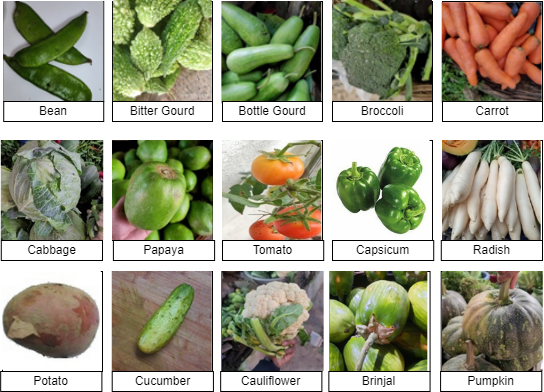
\includegraphics[width=\textwidth]{pic culinary vegetable}
\caption{Culinary vegetable }
\label{}
\end{figure}

Let’s say  $V={V_i, y_i }_(i=1)^k$ is a collection of RGB images that have been taken. Where, $V_i $represents the corresponding label for each $ i^{th} $  image in the collection, denoted by$ y_{i} \epsilon Y$ i.e,., $Y ={ y_i }_(i=1)^k For i={1,2,3,\dots k}$ and The dataset's instance count is determined by the constant k. each image is represented by a $M \in R^{(h×w×b)}$ a 2D (two-dimensional) matrix. The value in the matrix M, i row, and j column is indicated by $V_i \in V, M_{ij}$. H, W, or b indicate the batch size, height, and width. The scaled dataset  $\left\{V_i^t,y_i \right\}_{i=1}^k$  Required can be created using the resized function $fx()$ mentioned in equation \ref{equ1}.
\begin{equation} \label{equ1}
v^t=fx(\left\{V_i^t,y_i \right\}_{i=1}^k , p*q)
\end{equation}
% Main text

\begin{figure}
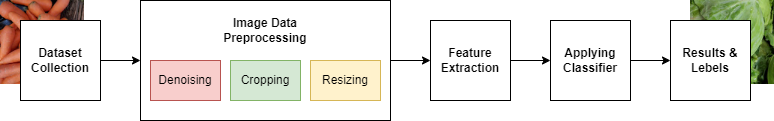
\includegraphics[width=\textwidth]{pic}
\caption{Model Architecture }
\label{}
\end{figure}

\begin{figure}
\centering
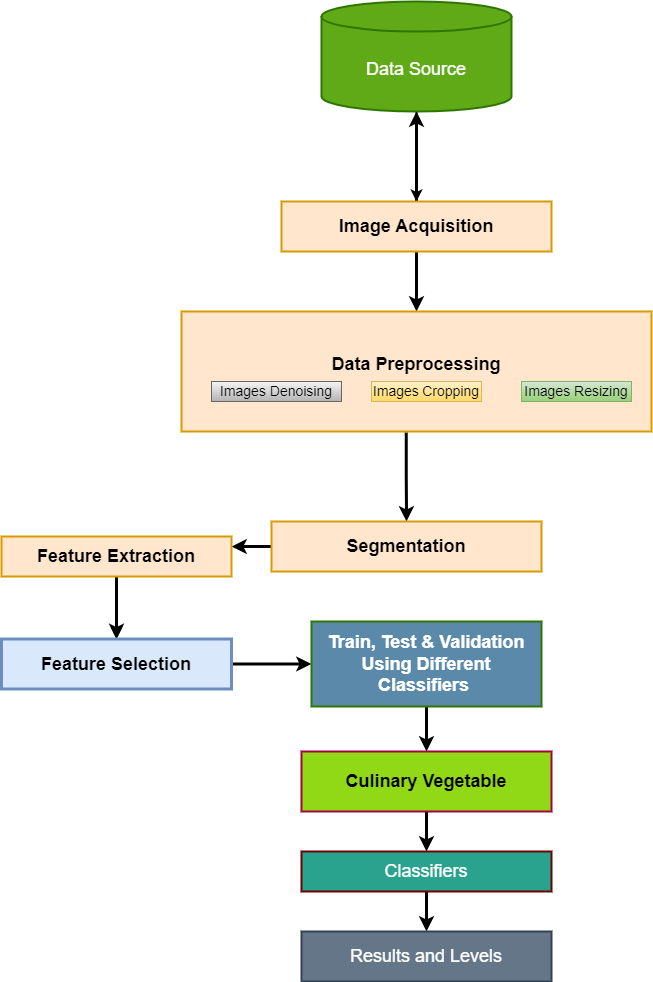
\includegraphics[scale=0.5]{flowchart}
\caption{Flow Chart Classification of Culinary Vegetables }
\label{}
\end{figure}

\subsection{PCA-based Feature Extraction}
\par To extract data from the images, principal component analysis (PCA) is employed \cite{wu2018review}. Then, the unnecessary information is removed without losing the vital information. The amount of data is reduced, which requires the machine to work less and learn more quickly, assuming that (m-1) is the principal component and that the greatest Eigenvalue of (m-1) is connected to Eigenvectors. component where the greatest Eigenvalue of (m-1) connects two eigenvectors. Subtraction of (m-1). Takes place for the principal component which is represented as. (m-1) is subtracted ,where $(b_1 \dots ,b_(m-1))$ is the representation of the $(m^{th})$ major component. Other elements reduce the remaining information. A new matrix, eq.\ref{equ2}, is produced as a result.
\begin{equation}\label{equ2}
\hat{X}=X- \sum_{i=1}^{m-1} b_1b_i^t X=X-B_{m-1}X
\end{equation}
          
    Where $[x_(1,)…….,x_(n])  \in R^(D×N)$ Where data points are used to represent column vectors and $B_(m-1)=x-\sum_{i=1}^{m-1} b_i b_i^T$. This project matrix shows the sunspace that is covered by $b_(1 \dots,b_(m-1) )$

\subsection{The dataset is split into the Test, Train, and Validate sections}
The dataset must be shuffled in the initial phase before being used for training, validating, and testing the split \cite{joseph2022split, goos2003d, berk1984validating}. Each class image is divided into three steps by the algorithm: training, validation, and testing. While the validation and test set each include 15\% of the photos from each category, the training set has 70\% of them. Let $ X=(X_1,\dots X_p)$ be the dataset, and k be the sample count. It is  $V^t$ The test dataset is divided into the test, train, validation, and test datasets, which are expressed as $T_{train} \subset V^t,V_{validation} \subset V^t and T_{test} \subset V^t$. Where $V^t=T_{train}\cup V_{validation}\cup T_{test} and {T_{train} \cap V_{validation} }\cup {T_{train}\cap T_{test} } \cup {V_{validation}\cap T_{test} }=\varnothing $ Considerations for the tensor include the RGB input image's height (h), width (w), and channel (c). The $i^{th}$  image of the dataset ${V_i^t\in V^t }$ can be expressed as
 $V_i^t=[H,W,C,i]$, where $i \in {1,2,3, \dots,b}$ and b is the batch size as shown in the equation	                  
\begin{equation}
X_t,Y_t
\end{equation}
  When the training portion of the data is designated as $X_t$ and the testing portion as$ Y_T $


\subsection{Analysis of Datasets Using Deep Learning Models After Training and Selection}
\textbf{Convolutional Layer:} During the convolution process, the kernel is required to modify the input[25]. Four-order tensors' kernel sizes could be represented as $H × W × C^l × C$ at the $I_{th}$ layer. The size of the convolution for the input  $H × W × C^l ×  b$  will be  $(H^l-H + 1) × (W^l- W + 1) × C$. Then, the convolutional method can be represented as an equation.4
\begin{equation}
y(i^{l+1},j^{l+1},k,b)=\sum_{i=0}^H \sum_{j=0}^w \sum_{k^{l=0}}^{c^l}W_{i,j,k^l,b}*x(i^{l+1},j^{l+1},k^{l,b})
\end{equation}
where $x(i^{l+1},j^{l+1},k^{l,b})$ denotes the element $x^l$ at the $l^{th}$ layer. Equation (4) is iterated $\AE 0 \leq c \leq C = C^{l+1}$ Pooling Layer: There are no parameters for the pooling process, i.e., $w^l = null$. The input's spatial range $X^l \in H^l × W^l × C^l × b$.   is the $I^{It}$ layer of  pooling[26]. The pooling output $X^{l+1} \in H^{l+1} × W^{l+1} × C^{l+1} × b$ will  be calculated as $H^{l+1} = H^l/H , W^{l+1}=\frac{w^l}{W} ,C^{l+1}=C^\frac{1}{C} $. 

It moves in both horizontal and vertical directions, although across a smaller area than $H×W$.                                   To see how the flattened layer fits within a standard CNN design, let's walk through it:
\begin{itemize}
\item Input layer: An image or feature map obtained from the layer before serves as the CNN's typical input.
\item Activation layers: An activation function (like RELU) is added to the network after each convolutional layer to increase nonlinearity\cite{o2015introduction}.
\item Pooling layers: By reducing the spatial dimensions of the output, pooling layers increase the network's computational efficiency and decrease its propensity for overfitting \cite{gholamalinezhad2020pooling, zafar2022comparison, zeiler2013stochastic}\\
\item Flatten layer: The final result is often a 3D tensor with dimensions (height, width, and channels) after we have completed the appropriate convolutions and pooling. This 3D tensor is flattened into a 1D vector, which is then used as the input for the succeeding fully connected layers.
\item Layers that are entirely connected: These layers connect each neuron in the current layer to each neuron in the layer above. Based on the collected features, high-level reasoning and decision-making are conducted using the fully linked layers.
\item Output layer: There usually are as many neurons in the last fully linked layer as classes in the classification task. The network's output is run through an appropriate activation function (such as softmax for multi-class classification) to create the final predictions.
\item Fully connected layer::. Convolutional layers only use the lth layer input value $x^l$  to calculate the $l^{th}$   layer output value $(l+1^{th})$. The fully connected layer, however[27], the output y, i.e., $x^{l+1} \in R^D$ with tensor panagakis2021tensor size ${H^l×W^l×C^l ×b}$, requires all input values $(i.e.,{x^l})$ from the $l^{th}$  levels that came before it. As can be seen below, the convolutional layer output from equation 5 can be used to express the final production at the $l^{th}$ layer \cite{basha2020impact}.
\end{itemize}
 \begin{equation}
	YL=\sum_{i=1}^{H}\sum_{j=1}^{w}\sum_{k^L=1}^{H} w_{i,jk^L,b*x_{(i^{L+1},j^{L+1}+j,k^L,b)}}
\end{equation}
Let F represent a network architecture function with bias, hyperparameters, learning rate, and other features.   Examples of  $\forall f \in F$  parameters that may be acquired after training on suitable training datasets include weights and biases. To produce the best-fit network with the least amount of overfitting or underfitting, however, finding the perfect function $f X \in F$ (with optimal parameters) is essential. Equation 6, which connects dataset X and labels y, can be used to express the optimum function.




\begin{equation}
	f*=argmin(\mu (X,y,f),subject of \in F)
\end{equation}
As a result, the model selected for a particular network is $f*$. There is also a more advanced architecture available as $f_F* \notin F$.
\begin{itemize}
\item Rectified Linear Unit (ReLu) layer: This layer increases the nonlinearity of the convolution neural network and has no learnable parameters. [28]. For every component of input, it truncates the data as $x_{i,j,k,b}^{l+1}=max\left \{0, x_{i,j,k,b}^{l} \right \}$ where $H^{l+1} =0  \leq i \leq H^l,W^{l+1} = 0 \leq i \leq W^l,C^{l+1}=0 \leq i \leq C^l$,and $B^{l+1}=0\leq b \leq B^l$.
\item Backward propagation: There are two sets of gradients needed for error backpropagation $\frac{\partial_z}{vec({x_i^l})} $ for input $x_i^l$ at the $l^{th}$ layer and partial derivatives of z controlled by $\omega^l$, such that,$\frac{\partial_z}{\partial_{vec({x^l})}}$. Consequently, convolution parameters may be used to define the parameters update rule in the $l^{th} $ layer. i.e.,$\phi{X^l }^T$, and transmission of a monitoring signal from layer ${l+1}^th$ layer, i.e., In the equation   $\frac{\partial_z}{\partial_{x^{l+1}}} $ Is indicated \cite{agarap2018deep, agarap1803deep}.
\end{itemize}
\begin{equation}
	\frac{\partial_z}{\partial_{vec}(\omega^l)}=\phi(X^l)^T*\frac{\partial_z}{\partial_{x^{l+1}}}
\end{equation}


\begin{figure}
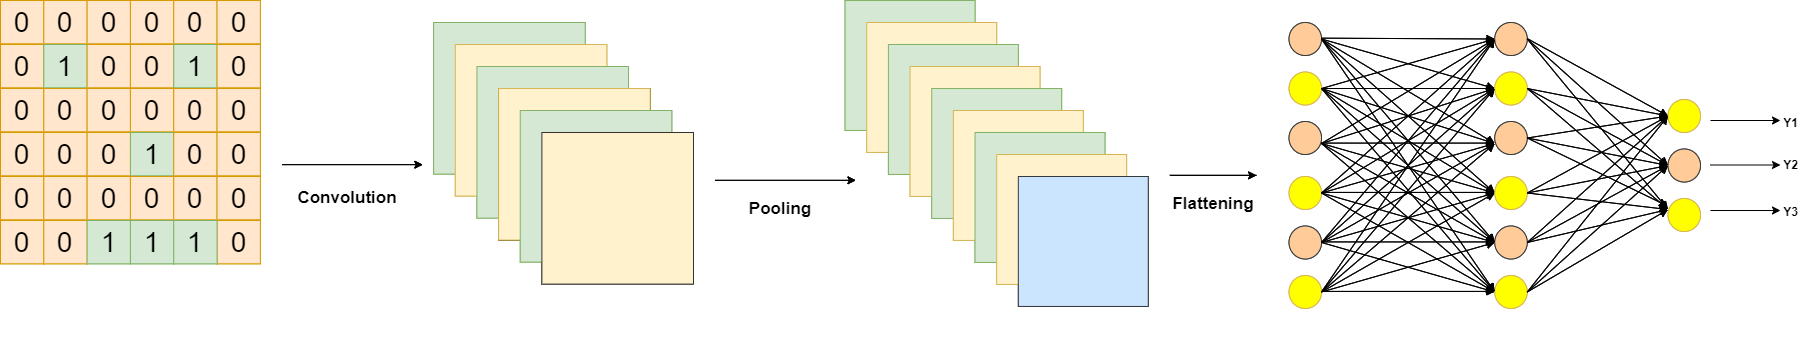
\includegraphics[width=\textwidth]{deep learning model}
\caption{Deep learning model training selection}
\label{}
\end{figure}

\section{Experiments}
 There are 21000 RGB images of culinary vegetable in total in the collection data, which are divided into 15 classes of culinary vegetable images. As shown in figure1., numerous types of vegetables with culinary vegetable were used in this research, including   brinjal, cauliflower, bean, bitter gourd, cabbage, potato, bottle gourd, broccoli, carrot, papaya, capsicum, pumpkin, cucumber, tomato and radish. There are a minimum of 850 images in each class. During the experiments, these images in each category are taken on a white background to eliminate anonymous or unusual data. the table contains a thorough dataset description, which includes a sample image of each class and their common name and a number of the sample image in each class, directly below each sample image. The algorithm divides each class image into three sections: Training, Validation, and Test. The training set comprises remaining more than 3000 images in each category, and the validation and test set each contains 6000 images.

\subsection{Experiment setup}
Figure 1 shows the experimental flowchart for the image of a culinary vegetable, which details the complete process from data collection to culinary vegetable categorization. The first phase of data collection for this study involved gathering a minimum of 850 photos of culinary vegetables from each of the 1 categoriesAfter gathering the dataset from various sources, it is pre-processed, including image cropping and maintaining sizeImages are resized to 224 X 224 in order to be evaluated. The pictures are presented in RGB format. The pictures were taken with a 16MP smartphone camera. The process is cluster-based. After feature extraction, the cluster-based technique provides us with a better outcome. It extracts picture properties and aids in providing an accurate result for the classifier. Resnet, Alexnet, Vgg, squeezenet, googlenet, shufflenet, resnext50, and densenet are the classifiers employed in this case. The accuracy of the classifiers is used to gauge their performance.  

\begin{figure}[!ht]
\centering
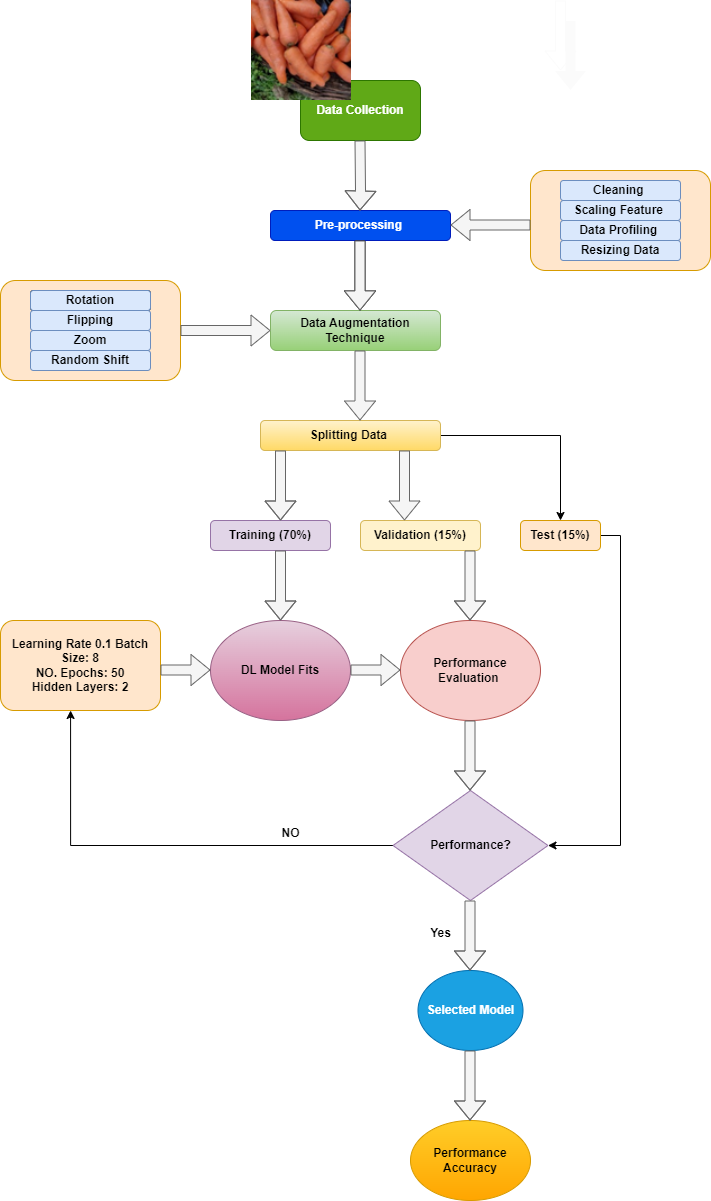
\includegraphics[scale=0.5]{Proposed model Architecture}
\caption{Proposed Model Architecture}
\label{}
\end{figure}


\subsection{Hardware and Software Requirement}
System Requirements: The following hardware and software have been employed in research: Our high-level programming language is Python 3.9.7 64-bit, our IDE is Anaconda Navigator 2.1.1, and it runs on the Google Collaboration Platform utilising a Jupyter Notebook 3.2. It also has a Quadro RTX 4000 GPU and Windows 10 as its operating system. The dataset is split into three equal halves for training, testing, and validation: 70\%, 15\%, and 15\%. For each dataset in this experiment, the same parameter values are utilised, and the effectiveness of each classifier is evaluated. Throughout the procedure, an HP Z6 G4 workstation was used.


\section{Description of results}
Heat-Map Confusion Matrix in Fig. 2. is the confusion matrix for the culinary vegetable dataset \cite{fernandez2017clustergrammer, soler2022data} using a heat map. The rightmost side has a scale from 0 to 0-4.5 that displays the correlation between the various classifiers. The two variables are significantly connected if the value is high or the scale value is 4.5. In a similar vein, there is no association between the two variables if the scale is low or 0. In fig. 2, we now. The output actually produced and the expected output are both accurately predicted because of the diagonal's strong correlation. Although the classifier did a decent job of classifying the data, many misclassifications occurred if the diagonal cells' colour was darker (closer to 0). However, the narrative will be completely the opposite save for this diagonal cell. That is much darker (nearer to 0). The colour indicates that there is an association between that class and the corresponding other culinary vegetable classes \cite{read2011classifier, read2009classifier}

\begin{figure}[!ht]
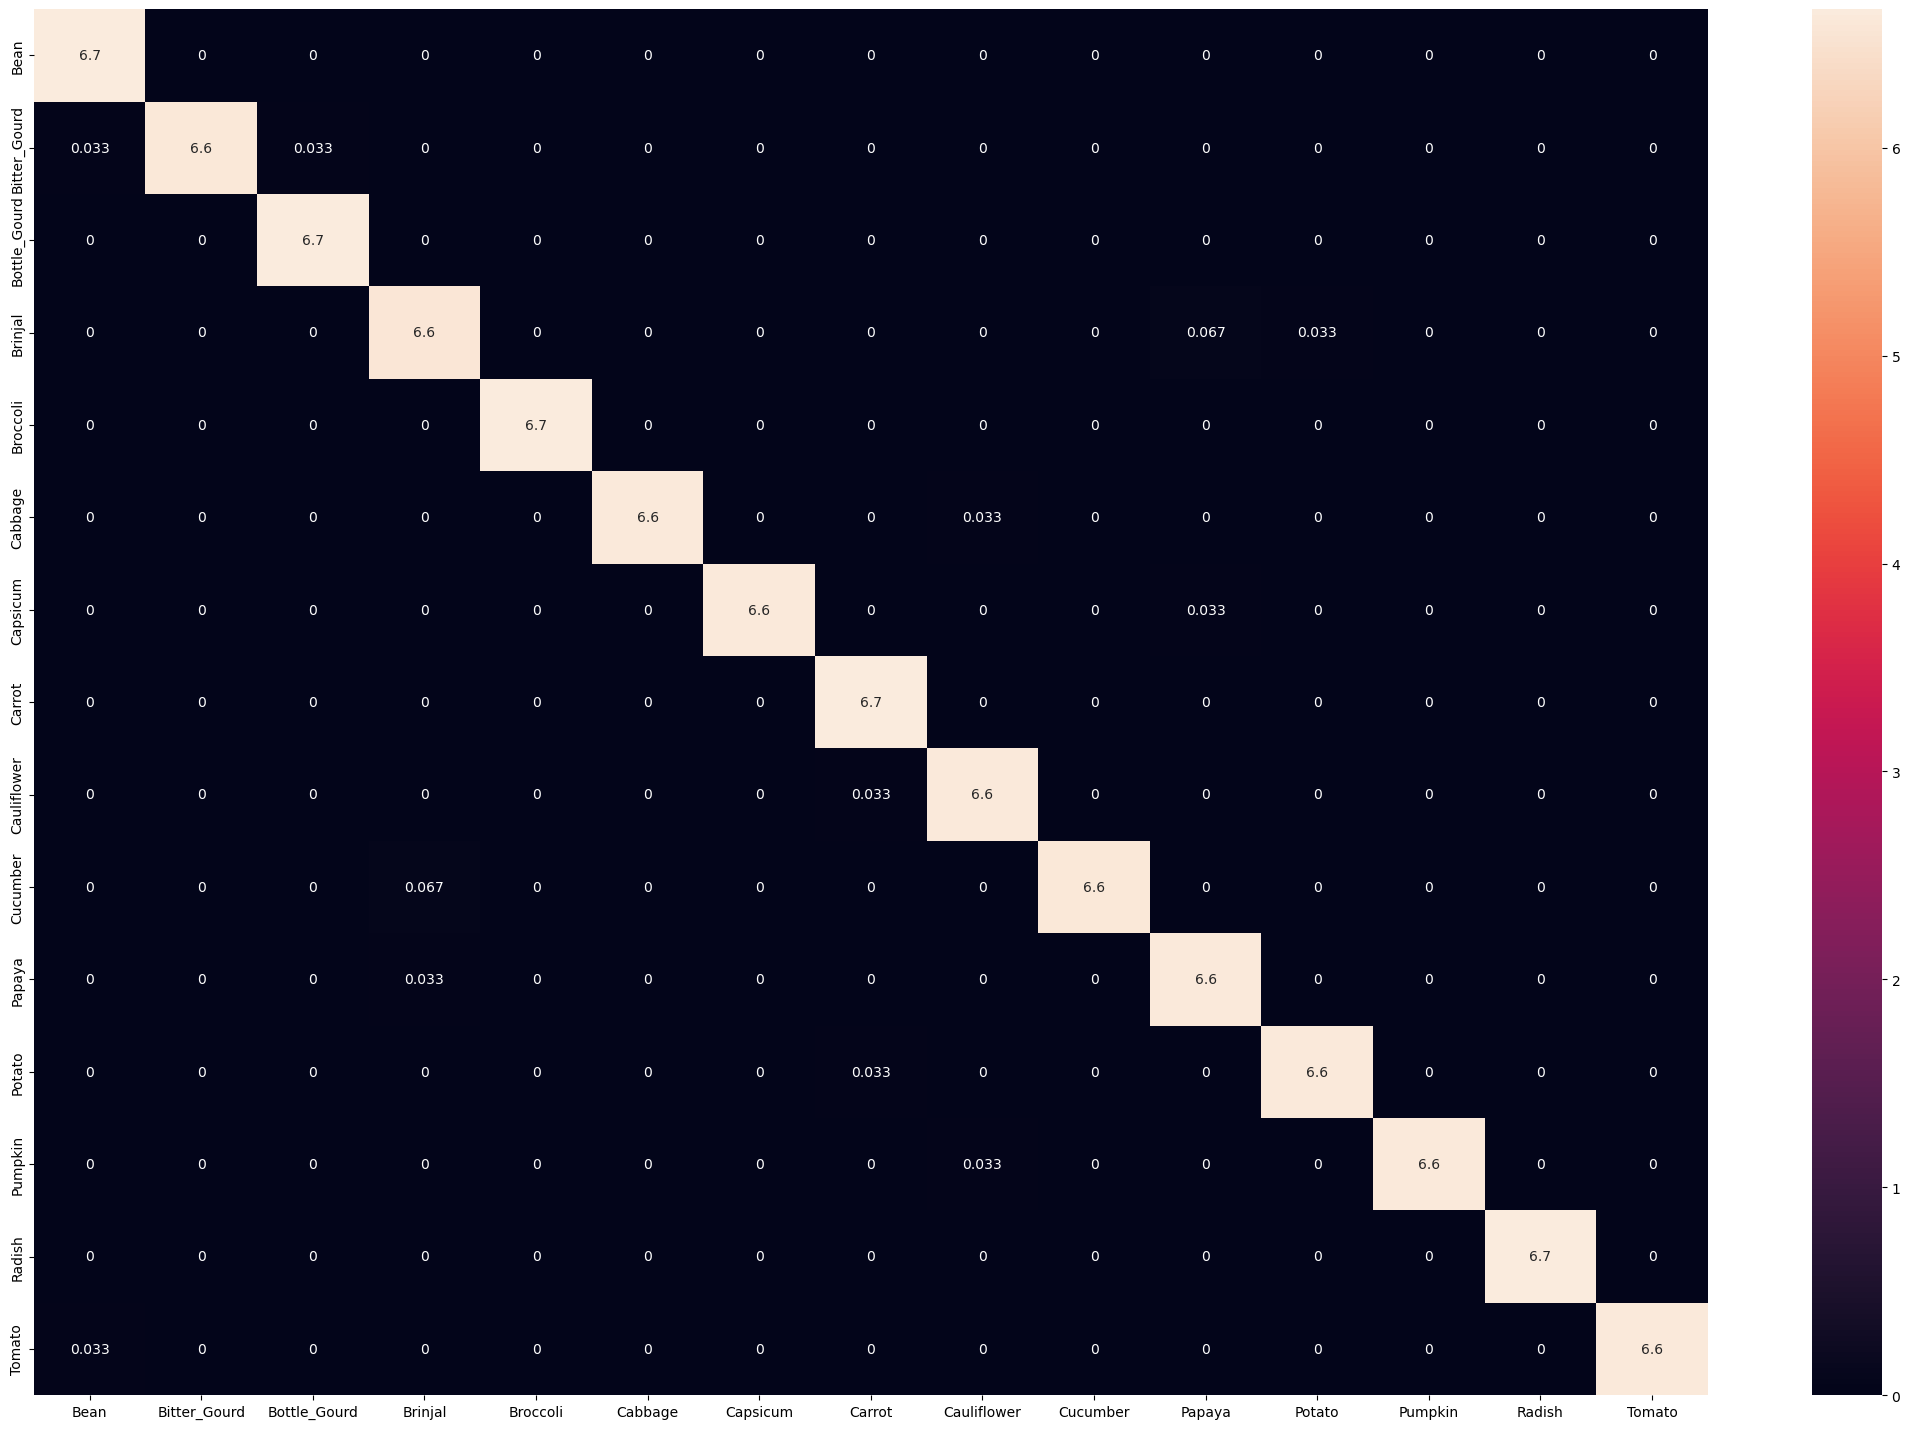
\includegraphics[scale=0.3]{correlation Matrics}
\caption{Confusion Matrix Using Heatmap Of Classifiers}
\label{}
\end{figure}



\begin{figure}[!ht]
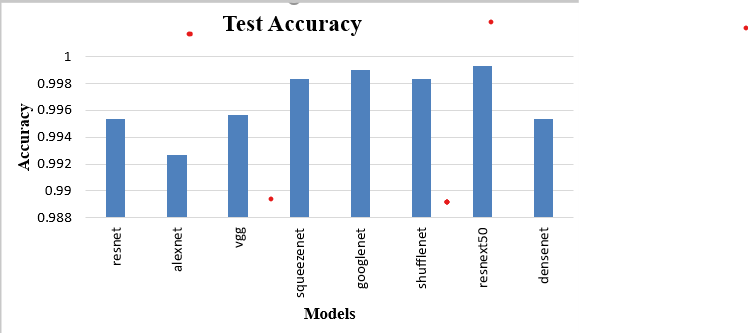
\includegraphics[scale=0.75]{test Accuracy}
\caption{Test Accuracy of All Models}
\label{}
\end{figure}
%\begin{figure}

\begin{figure}[!ht]
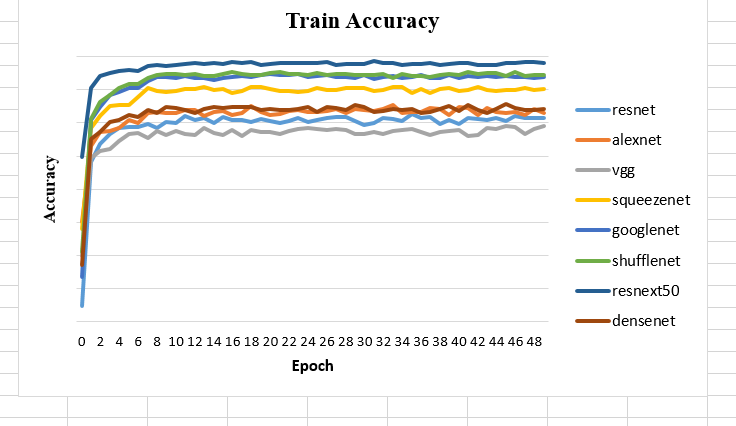
\includegraphics[scale=0.75]{Train Accuracy}
\caption{Train Accuracy of All models With  Corresponding Epochs}
\label{}
\end{figure}

\begin{figure}[!ht]
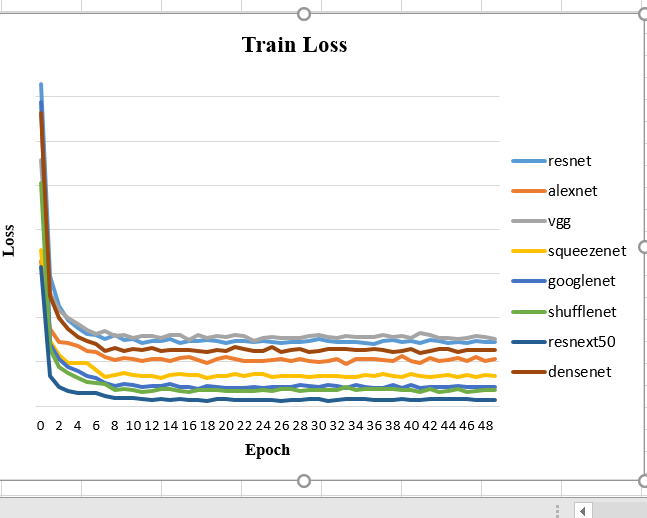
\includegraphics[scale=0.75]{Train Loss}
\caption{Train Loss of All Models With corresponding Epochs}
\label{}
\end{figure}

\begin{figure}[!ht]
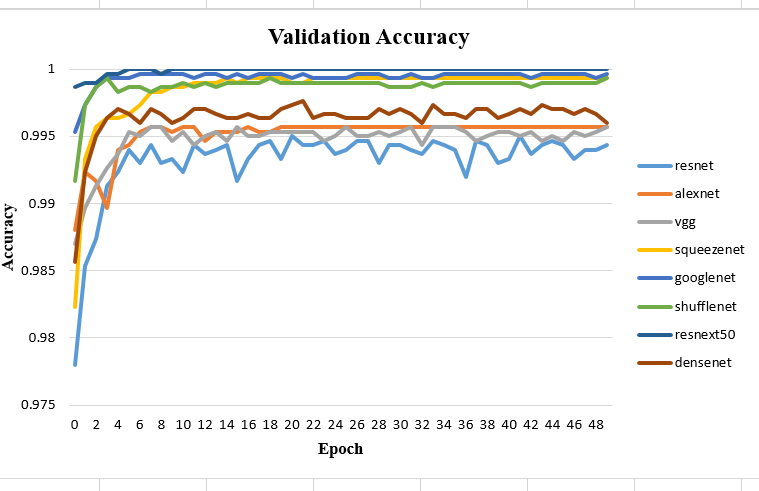
\includegraphics[scale=0.75]{Train validation Accuracy}
\caption{Validation Accuracy of All models with corresponding Epochs}
\label{}
\end{figure}

\begin{figure}[!ht]
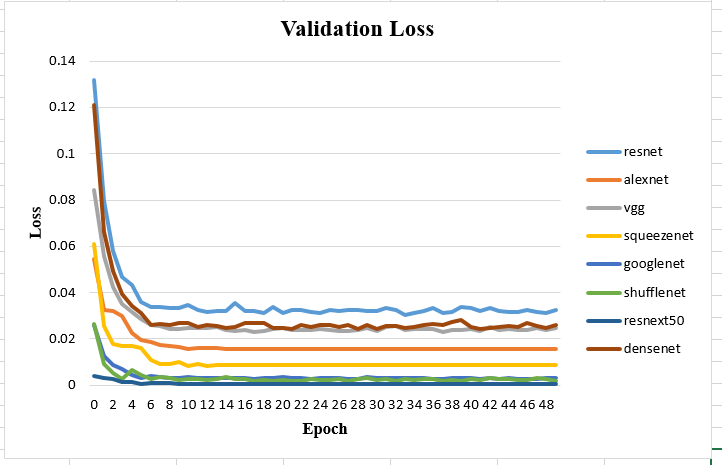
\includegraphics[scale=0.75]{validation loss}
\caption{Validation loss of All Models With corresponding Epochs}
\label{}
\end{figure}





\section{Analysis of Results}
ResNet18 is the name given to the 18-layer ResNet design. It is well recognised for incorporating skip connections, commonly referred to as residual blocks, which solve the vanishing gradient problem and make it appropriate for deep networks. A completely linked classification layer makes up the final layer of the model. AlexNet is a state-of-the-art deep neural network architecture. This approach uses convolutional layers that are completely coupled. It was crucial for the widespread application of deep learning to photo classification issues. Convolutional layers are stacked, and then max-pooling layers are added to construct the VGGNet's uniform $ VGG11$bn enhances training stability. With fewer parameters, SqueezeNet is intended to be a small deep neural network architecture. The model is accurately maintained while being compressed using 1x1 convolutions and fire modules. A well-known aspect of DenseNet is its dense connectivity between layers. It creates feedforward connections between each layer to promote gradient flow and feature reuse. GoogleNet, also known as Inception v1, was the business that originated the concept of inception modules. It aims to be both computationally efficient and insightful. It is effective for a variety of picture categorization tasks. To balance model accuracy and processing speed, ShuffleNet employs channel shuffling and group convolutions. It performs admirably for real-time applications on hardware with limited resources.ResNeXt is a supplement to the ResNet architecture. The addition of cardinality improves the model's usability. ResNeXt50\_32x4d describes the network depth and cardinality settings.





\section{conclusion}
Image processing is used to classify the various 15 categories of culinary vegetable images. For each of the 15 classes of vegetable, minimum of 850 pictures were painstakingly collected. As a result, the dataset used in this study is unique. To begin the categorization, the shape feature is extracted. Second, several approaches such as Resnet, Alexnet, Vgg, Squeezenet, Googlenet, Shufflenet, Resnet50 and Densenet and were used to obtain classification accuracies. Based on these findings, the analysis was drawn using heat maps. Using the Resnet50 Classifier of the Deep Learning model, it’s obtained an accuracy of 0.998\%. The farmers will get benefited directly after the implementation of this model in-app. This will boost the farming sector, leading to a boost in the Indian economy. Through this paper, it is seen that Resnet50 classifiers performed better than any other classifier. I have used eight classifiers and analyzed their performance through accuracy. For visualization, I used a heat map, which gives us a clear view of their classifier performance. I finalized this result by doing hyperparameter tuning and each classifier and checked their best effect.

In the future, the Machine learning model will be applied to the same dataset of 15 different culinary vegetable to achieve higher accuracy than the best Ma- chine learning model, and the correlation of some culinary vegetable, such as LIMA BEAN, TOMATO, POTATO, and others, will be improved through proper data analysis. Other algorithms can also be evaluated to choose the best classifier. Deep learning and other advanced methods can be utilized for severely misclassified categories. More culinary vegetable image categories can be collected for classification.






\section*{CRediT authorship contribution statement}
\textbf{Chandan kumar}:Software , Data Curation, Methodology, Writing - Original Draft preparation, Visulization
 
\section*{Data availability}
This project's culinary vegetable image collection was sourced from Kaggle, a well-known website for sharing and accessing datasets. Datasets for computer vision and machine learning challenges are among the many datasets Kaggle is renowned for hosting. The following features are present in this dataset, which was especially selected for culinary vegetable classification.
A great place to find a dataset of culinary vegetable images appropriate for deep learning model training is Kaggle. This dataset can be used by academics and industry professionals interested in creating and assessing vegetable categorization algorithms to build and test deep learning models, ultimately advancing culinary computer vision applications. To ensure correct usage and adherence to licencing agreements, it is crucial to review the precise terms and conditions linked with the dataset on Kaggle.
\section*{Acknowledgments}
\label{}






\label{}

% To print the credit authorship contribution details
\printcredits

%% Loading bibliography style file
%\bibliographystyle{model1-num-names}
\bibliographystyle{cas-model2-names}

% Loading bibliography database
\bibliography{ref}

% Biography
\bio{}
% Here goes the biography details.
\endbio

%\bio{pic1}
% Here goes the biography details.
\endbio

\end{document}

